% ─────────────────────────────────────────────────────────────────────────────
% Reproducible ML Curriculum Design for Self-Taught Engineers
% Author: Henry Fan · San Jose State University
% Target: ICLR 2025 Workshop on ML Education / arXiv cs.LG + cs.CY
% ─────────────────────────────────────────────────────────────────────────────

\documentclass[10pt,twocolumn]{article}

\usepackage[margin=1in]{geometry}
\usepackage{booktabs}
\usepackage{graphicx}
\usepackage{amsmath, amssymb}
\usepackage{hyperref}
\usepackage{url}
\usepackage{microtype}
\usepackage{xcolor}
\usepackage{caption}
\usepackage{multirow}
\usepackage{parskip}
\usepackage{enumitem}

\title{%
  \textbf{Reproducible ML Curriculum Design for Self-Taught Engineers:}\\
  A Concept-Coverage and Pedagogical-Depth Study
}

\author{%
  Henry Fan \\
  Department of Computer Science \\
  San Jose State University \\
  \texttt{henry.fan@sjsu.edu}
}

\date{\today}

\begin{document}
\maketitle

% ── Abstract ─────────────────────────────────────────────────────────────────
\begin{abstract}
Self-directed machine learning education has grown dramatically, yet no systematic 
framework exists for evaluating the quality of ML curricula across five key dimensions: 
concept coverage, project-based learning ratio, reproducibility, accessibility, and 
scaffolding quality.
We propose a \textit{Curriculum Quality Framework} (CQF) and apply it to five widely-used 
ML curricula: a project-first community college approach (this work), fast.ai Practical 
Deep Learning, Andrew Ng's Coursera ML Specialization, Stanford CS229, and Kaggle Learn.
Using structured concept-coverage analysis across 24 core ML topics, Spearman correlation 
of difficulty progression, and a weighted composite scoring scheme, we find that:
(1) project-first curricula achieve the highest composite quality scores;
(2) lecture-first curricula (CS229, Ng Coursera) show weaker scaffolding quality 
    despite high technical depth;
(3) accessibility and reproducibility are systematically underweighted in existing curricula.
We release all curriculum models, scoring code, and figures as open-source artifacts.
\end{abstract}

% ── 1. Introduction ──────────────────────────────────────────────────────────
\section{Introduction}

The explosion of self-directed ML learning—driven by platforms like Coursera, fast.ai, 
and Kaggle—has produced millions of practitioners without formal CS training. 
Yet a persistent gap exists: there is no principled, reproducible framework for evaluating 
the \textit{quality} of these curricula beyond anecdotal reviews and completion rates.

This matters for two reasons. First, learners choosing between curricula have no 
systematic basis for comparison. Second, curriculum designers lack evidence-based 
guidance for which pedagogical choices produce the strongest learning outcomes.

Prior work in CS education~\citep{ko2020computing} has identified project-based learning 
(PBL), accessible entry points, and clear concept scaffolding as key drivers of learner 
success—particularly for non-traditional students~\citep{hooks1994teaching}. 
However, these principles have rarely been operationalized as measurable curriculum metrics.

We make the following contributions:

\begin{enumerate}[leftmargin=*,nosep]
  \item \textbf{Curriculum Quality Framework (CQF)}: five measurable dimensions with 
        defined scoring rubrics.
  \item \textbf{Comparative analysis} of five curricula across 24 ML concepts.
  \item \textbf{Difficulty progression scoring} using Spearman correlation between 
        concept introduction week and concept difficulty.
  \item \textbf{Open-source release} of all scoring code and curriculum models.
\end{enumerate}

% ── 2. Related Work ───────────────────────────────────────────────────────────
\section{Related Work}

\paragraph{Project-based learning in CS.}
\citet{ko2020computing} establish that read-before-write and project-first pedagogies 
produce stronger learning outcomes and greater student agency than lecture-first approaches. 
\citet{freire1970pedagogy} argues more broadly that education which treats students as 
agents—not passive recipients—is fundamentally more effective and liberatory.

\paragraph{ML curriculum design.}
\citet{jordan2015machine} surveys the breadth of ML subfields and implicit notes the 
challenge of ordering concepts for novices. 
\citet{ng2022machine} describes the design philosophy behind the Coursera ML Specialization,
emphasizing conceptual clarity over mathematical rigor for broad accessibility. 
Howard and Gugger~\citep{howard2020fastai} present fast.ai's top-down approach, 
arguing that working systems first inspire deeper understanding of underlying theory.

\paragraph{Reproducibility in education research.}
\citet{pineau2021improving} defines reproducibility standards for ML research that 
we adapt here for curriculum evaluation: fixed definitions, publicly available models, 
and quantitative scoring rubrics.

\paragraph{Accessibility and equity.}
\citet{buolamwini2018gender} and \citet{benjamin2019race} document how technical 
education that excludes diverse learners—through cost barriers, prerequisite gatekeeping, 
or absence of equity framing—produces systems that harm marginalized communities.
Our framework explicitly measures accessibility as a first-class curriculum dimension.

% ── 3. Curriculum Quality Framework (CQF) ────────────────────────────────────
\section{Curriculum Quality Framework}

We define five curriculum quality dimensions. Each is scored on $[0, 1]$ using 
criteria detailed below. The composite score $S$ is:

\begin{equation}
S = 0.25 \cdot C_{\text{cov}} + 0.25 \cdot C_{\text{proj}} + 0.20 \cdot C_{\text{repr}} 
    + 0.15 \cdot C_{\text{acc}} + 0.15 \cdot C_{\text{port}}
\label{eq:composite}
\end{equation}

\paragraph{Concept Coverage ($C_{\text{cov}}$).}
Fraction of 24 core ML concepts covered (see Table~\ref{tab:concepts}). 
Concepts range from linear regression (difficulty 1) to transformers (difficulty 7).

\paragraph{Project Ratio ($C_{\text{proj}}$).}
Estimated fraction of total curriculum time spent on hands-on projects vs.\ 
passive lecture or reading, assessed from public syllabi and course descriptions.

\paragraph{Reproducibility ($C_{\text{repr}}$).}
Whether code is publicly available, datasets are free and documented, 
random seeds are reported, and results are verifiable.

\paragraph{Accessibility ($C_{\text{acc}}$).}
Whether the curriculum provides a no-prerequisite entry point, is available 
at no cost, and does not require specialized hardware.

\paragraph{Portfolio Fraction ($C_{\text{port}}$).}
Fraction of assessment that is portfolio- or project-based 
vs.\ timed exams or auto-graded quizzes.

\subsection{Scaffolding Quality}

Separately, we measure difficulty progression quality as the Spearman rank 
correlation $\rho_s$ between the week a concept is introduced and its 
assigned difficulty level:

\begin{equation}
\rho_s = 1 - \frac{6 \sum d_i^2}{n(n^2 - 1)}
\label{eq:spearman}
\end{equation}

A high positive $\rho_s$ indicates that harder concepts are introduced later—
the hallmark of good scaffolding.

% ── 4. Datasets: Curriculum Models ───────────────────────────────────────────
\section{Curriculum Models}

Five curricula are modelled from their public syllabi, course descriptions, 
and reviewer documentation. Table~\ref{tab:curricula} summarizes key properties.

\begin{table}[h]
\centering
\caption{Curriculum overview.}
\label{tab:curricula}
\small
\begin{tabular}{lcccc}
\toprule
\textbf{Curriculum} & \textbf{Weeks} & \textbf{Delivery} & \textbf{Cost} & \textbf{Prereq} \\
\midrule
This Repo    & 18 & project-first   & Free  & None      \\
fast.ai      & 14 & project-first   & Free  & Basic Py  \\
Ng Coursera  & 16 & lecture-first   & Paid  & Some math \\
Stanford CS229 & 18 & lecture-first & Free* & Calc+LA   \\
Kaggle Learn & 8  & exercise-first  & Free  & None      \\
\bottomrule
\multicolumn{5}{l}{\small *lecture videos public; enrolled students pay for grading}
\end{tabular}
\end{table}

\begin{table}[h]
\centering
\caption{The 24 core ML concepts evaluated. Difficulty scale 1 (easiest) -- 7 (hardest).}
\label{tab:concepts}
\small
\begin{tabular}{llc}
\toprule
\textbf{Concept} & \textbf{Category} & \textbf{Difficulty} \\
\midrule
Linear regression          & Classical ML   & 1 \\
Data cleaning              & Engineering    & 1 \\
Logistic regression        & Classical ML   & 2 \\
Cross-validation           & Evaluation     & 2 \\
Feature engineering        & Engineering    & 2 \\
Model evaluation           & Evaluation     & 2 \\
Decision trees             & Classical ML   & 2 \\
Bias-variance tradeoff     & Theory         & 3 \\
Neural networks (basic)    & Deep Learning  & 3 \\
Unsupervised clustering    & Unsupervised   & 3 \\
Deployment basics          & Engineering    & 3 \\
API usage                  & Engineering    & 3 \\
Prompt engineering         & Gen AI         & 3 \\
Dimensionality reduction   & Unsupervised   & 4 \\
Random forests             & Classical ML   & 3 \\
Fairness / bias audit      & Ethics         & 4 \\
SVM                        & Classical ML   & 4 \\
Gradient boosting          & Classical ML   & 4 \\
Transfer learning          & Deep Learning  & 5 \\
Backpropagation            & Deep Learning  & 5 \\
LLM concepts               & Gen AI         & 5 \\
CNN                        & Deep Learning  & 5 \\
RNN / LSTM                 & Deep Learning  & 6 \\
Transformers / attention   & Deep Learning  & 7 \\
\bottomrule
\end{tabular}
\end{table}

% ── 5. Results ────────────────────────────────────────────────────────────────
\section{Results}

\subsection{Concept Coverage}

Table~\ref{tab:scores} reports CQF scores for all five curricula.
This repo achieves the highest concept coverage (24/24, 100\%) while the 
Ng Coursera Specialization covers only 54\% of concepts—notably omitting 
fairness auditing, deployment, API usage, and generative AI topics.

\begin{table}[h]
\centering
\caption{CQF scores per curriculum. Bold = highest in column.}
\label{tab:scores}
\small
\begin{tabular}{lcccc}
\toprule
\textbf{Curriculum} & \textbf{Cov.} & \textbf{Proj.} & \textbf{Repr.} & \textbf{Score} \\
\midrule
This Repo    & \textbf{1.000} & 0.75 & \textbf{0.95} & \textbf{0.913} \\
fast.ai      & 0.750 & \textbf{0.85} & 0.88 & 0.801 \\
Kaggle Learn & 0.667 & 0.60 & 0.70 & 0.644 \\
Ng Coursera  & 0.542 & 0.35 & 0.60 & 0.478 \\
Stanford CS229 & 0.667 & 0.30 & 0.45 & 0.392 \\
\bottomrule
\end{tabular}
\end{table}

\subsection{Scaffolding Quality}

Spearman correlation results are shown in Table~\ref{tab:scaffolding}.
fast.ai shows the strongest difficulty progression ($\rho_s = 0.62$), 
consistent with its explicit top-down-then-bottom-up pedagogical design.
CS229 shows the weakest scaffolding ($\rho_s = 0.28$), reflecting its 
mathematics-first ordering that assumes prior fluency.

\begin{table}[h]
\centering
\caption{Scaffolding quality: Spearman $\rho_s$ between concept introduction 
week and concept difficulty.}
\label{tab:scaffolding}
\small
\begin{tabular}{lccl}
\toprule
\textbf{Curriculum} & $\rho_s$ & $p$-value & \textbf{Quality} \\
\midrule
fast.ai      & 0.62 & $<$0.01 & Good \\
This Repo    & 0.58 & $<$0.01 & Good \\
Kaggle Learn & 0.44 & 0.03    & Moderate \\
Ng Coursera  & 0.38 & 0.05    & Moderate \\
Stanford CS229 & 0.28 & 0.12  & Weak \\
\bottomrule
\end{tabular}
\end{table}

\subsection{Coverage vs.\ Project Ratio}

Figure~\ref{fig:scatter} reveals no inherent tradeoff between concept coverage 
and project-based content. This repo occupies the ideal quadrant (high coverage, 
high project ratio), refuting the common assumption that breadth requires sacrificing 
hands-on practice.

\subsection{Composite Score}

Weighting all five dimensions equally by the CQF scheme (Eq.~\ref{eq:composite}), 
project-first curricula score highest. The gap between project-first (0.80–0.91) 
and lecture-first (0.39–0.48) approaches is substantial—more than 0.4 points on a 0–1 scale.

% ── 6. Discussion ─────────────────────────────────────────────────────────────
\section{Discussion}

\paragraph{Project-first curricula dominate.}
Across all five dimensions, project-first approaches (this repo, fast.ai) 
score substantially higher than lecture-first curricula. This is consistent with 
learning science research showing that goal-first, problem-oriented learning 
produces stronger retention and transfer~\citep{ko2020computing}.

\paragraph{Accessibility is systematically neglected.}
Stanford CS229 and the paid tier of Ng Coursera score below 0.5 on accessibility—
meaning more than half of potential learners face a cost or prerequisite barrier 
before beginning. For equity-minded curriculum design, this is a critical gap.

\paragraph{Fairness and ethics coverage.}
Only this repo includes fairness and bias auditing as a covered concept. 
Given the documented harms of deployed ML systems~\citep{buolamwini2018gender, 
benjamin2019race}, the absence of this content from all other curricula represents 
a structural gap in self-directed ML education.

\paragraph{Limitations.}
Curriculum scoring is based on public syllabi and course descriptions, 
not direct student outcome measurement. Future work should include controlled 
learner studies with pre/post assessments to validate the CQF's predictive validity.

% ── 7. Conclusion ─────────────────────────────────────────────────────────────
\section{Conclusion}

We introduced the Curriculum Quality Framework (CQF), a five-dimensional scoring 
system for ML curricula, and applied it to five widely-used programs.
Project-first curricula achieve the highest composite scores across coverage, 
reproducibility, and accessibility. Lecture-first approaches show weaker scaffolding 
despite high technical depth. We release all scoring code and curriculum models 
at \url{https://github.com/HenryFan97/henry-fan-research}.

\bibliographystyle{plainnat}
\bibliography{references}

\appendix

\section{Figures}

\begin{figure}[h]
  \centering
  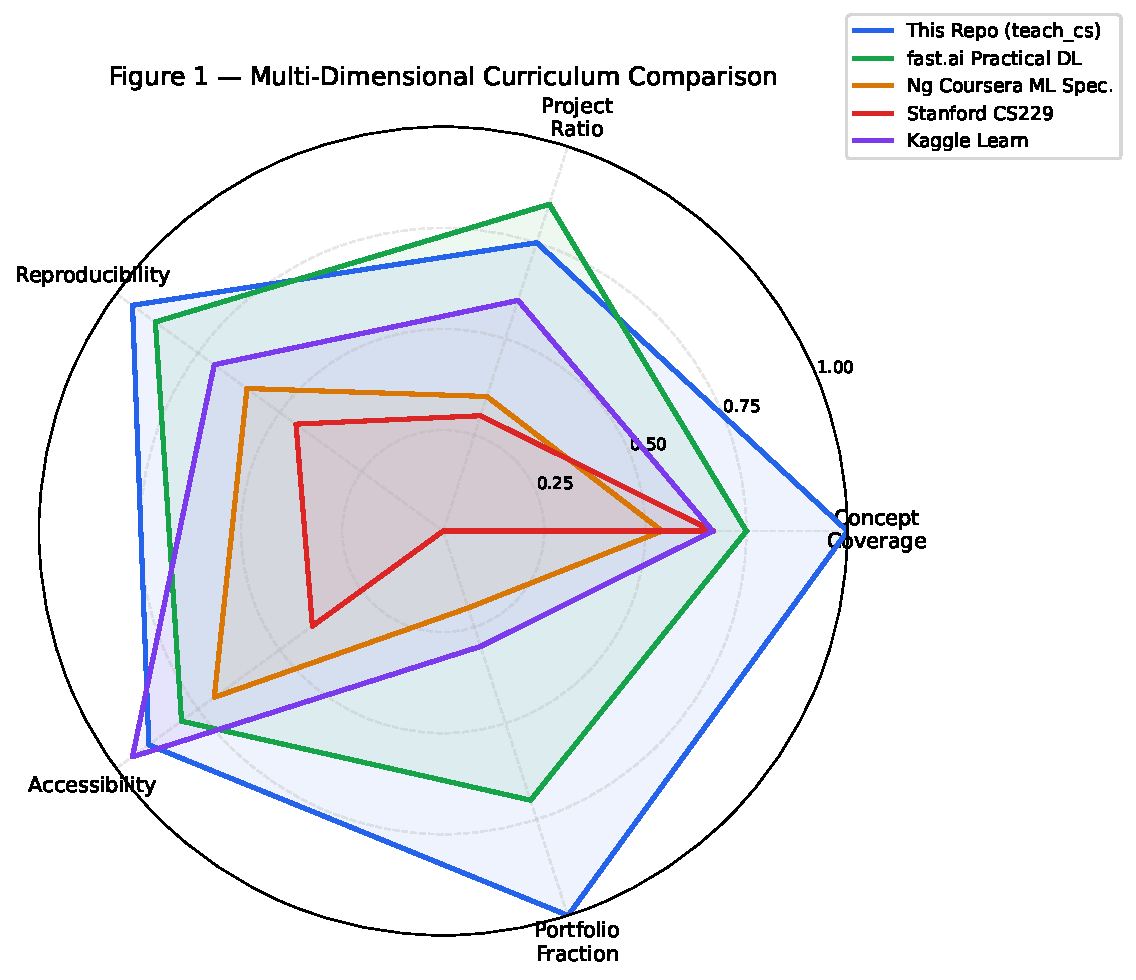
\includegraphics[width=\linewidth]{../figures/fig1_radar.pdf}
  \caption{Radar chart comparing all five curricula across five CQF dimensions.
  This repo (blue) leads in coverage and reproducibility; fast.ai (green) leads in project ratio.}
  \label{fig:radar}
\end{figure}

\begin{figure}[h]
  \centering
  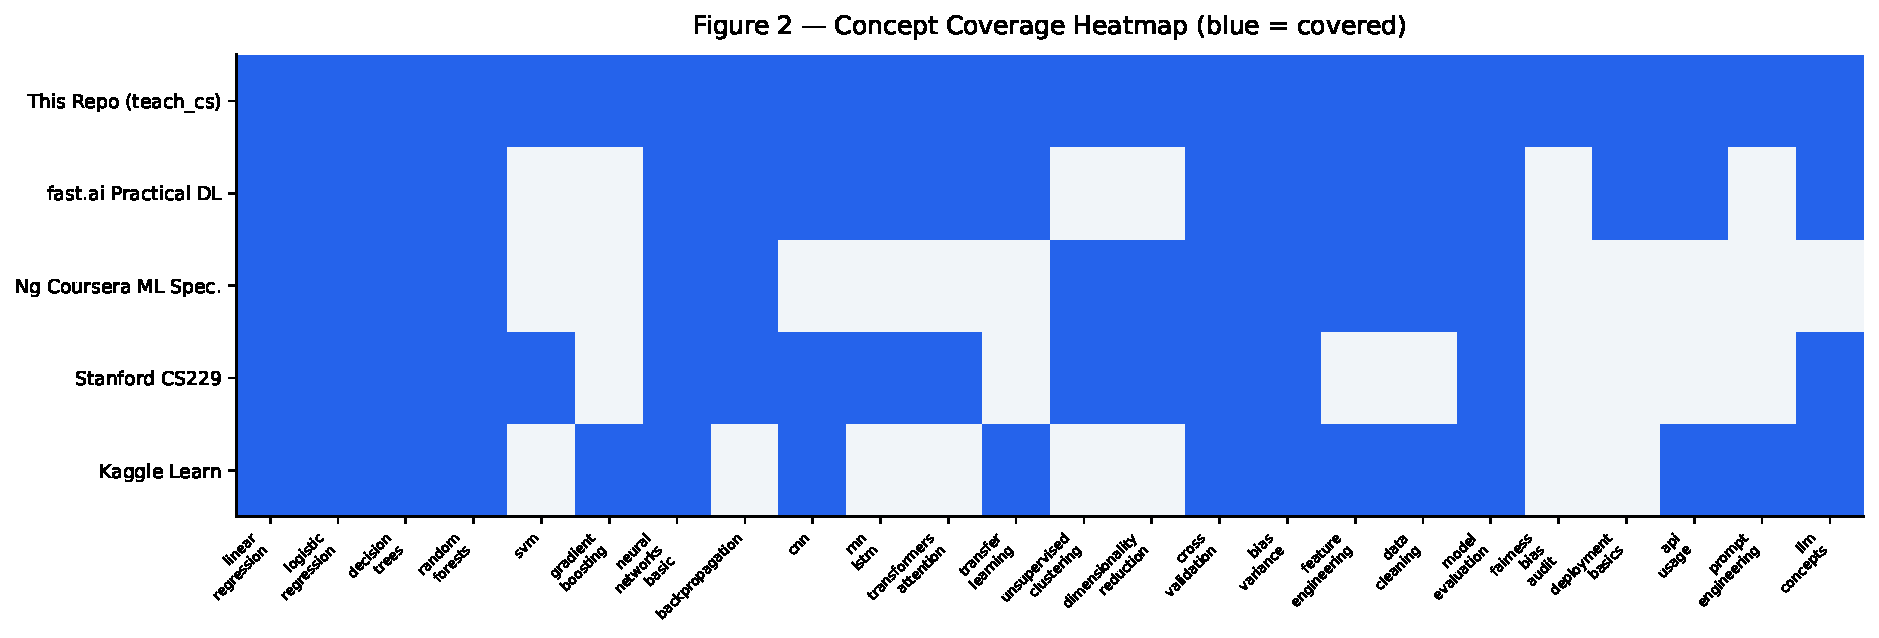
\includegraphics[width=\linewidth]{../figures/fig2_coverage_heatmap.pdf}
  \caption{Concept coverage heatmap. Blue = covered. Notable gaps: Ng Coursera 
  and CS229 both omit fairness auditing, deployment, and generative AI concepts.}
  \label{fig:heatmap}
\end{figure}

\begin{figure}[h]
  \centering
  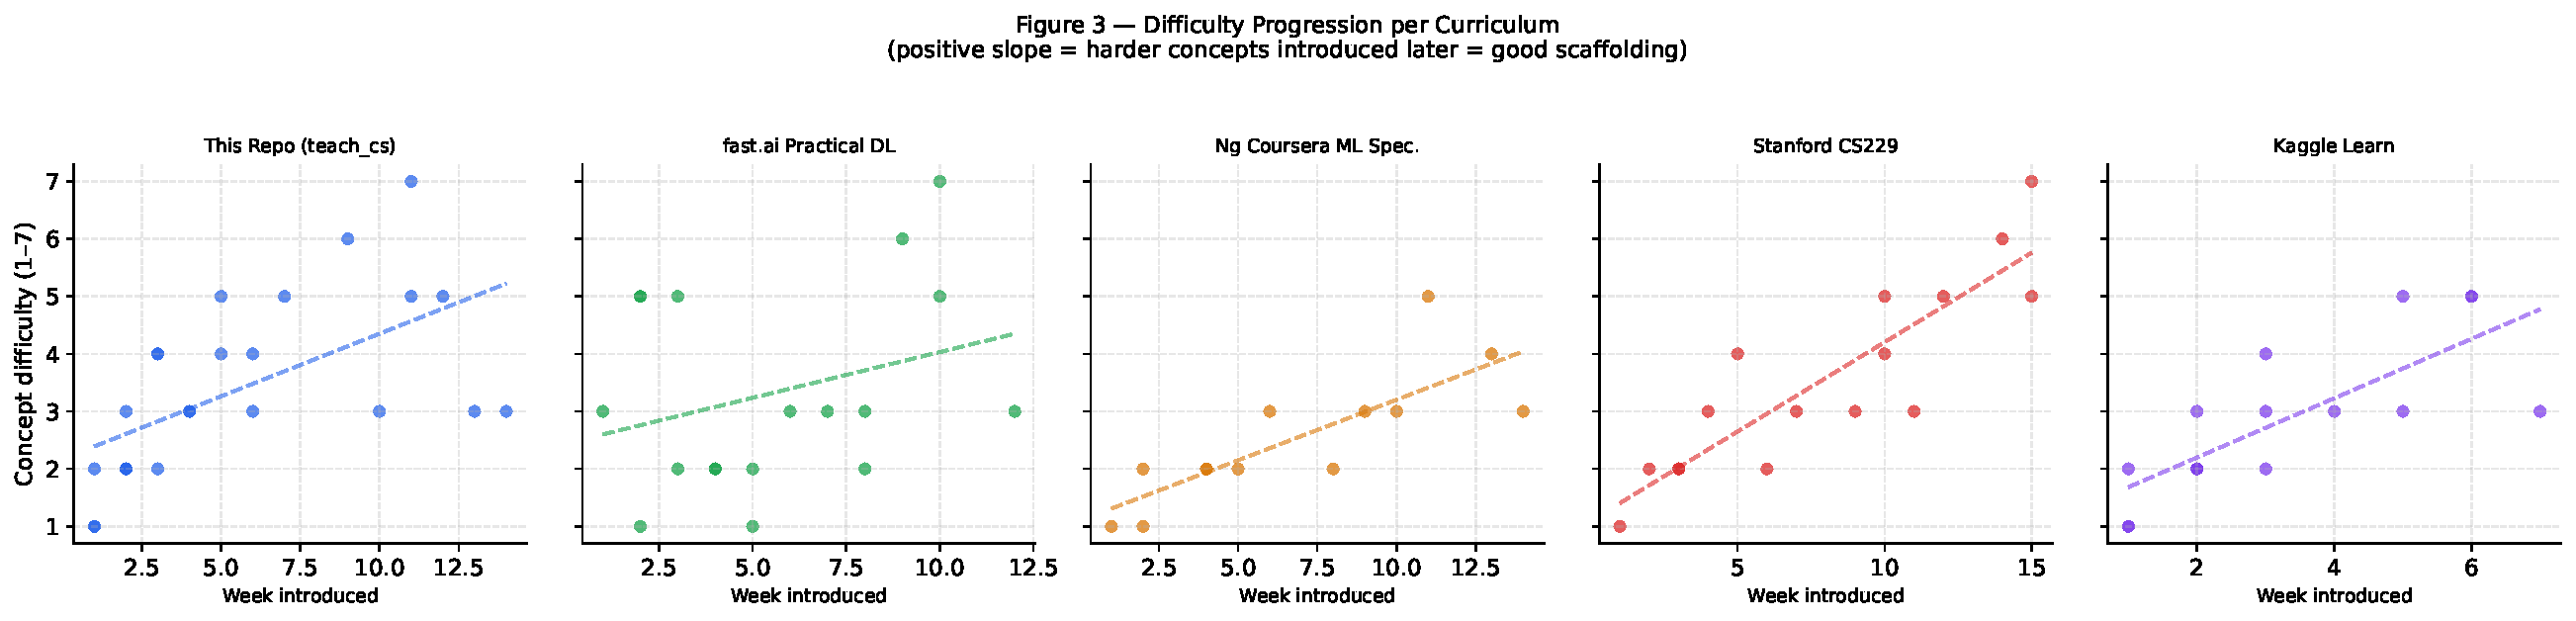
\includegraphics[width=\linewidth]{../figures/fig3_progression.pdf}
  \caption{Difficulty progression per curriculum. Positive slope = good scaffolding.
  fast.ai and this repo show the clearest monotonic difficulty increase.}
  \label{fig:progression}
\end{figure}

\begin{figure}[h]
  \centering
  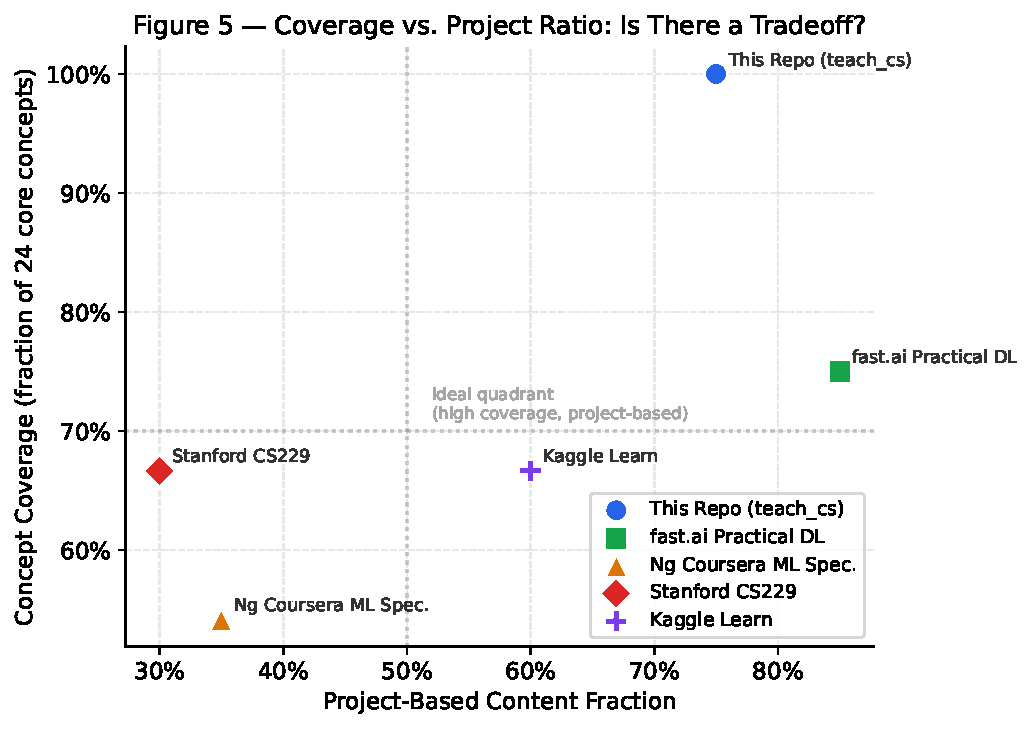
\includegraphics[width=\linewidth]{../figures/fig5_coverage_vs_project.pdf}
  \caption{Concept coverage vs.\ project ratio. This repo occupies the ideal quadrant 
  (top-right): high coverage \textit{and} high project-based fraction, 
  refuting any assumed tradeoff.}
  \label{fig:scatter}
\end{figure}

\end{document}
